\section{Varianten des gemeinsamen Wissens}
\label{GemeinsamesWissen}
In Kap. 4 wurden bereits asynchrone Systeme dargestellt. Dieses Kapitel behandelt Erweiterungen für asynchrone Systeme um einen Grad an Zuverlässigkeit zu gewährleisten. Die Prozesse müssen Vereinbarungen treffen. Dies bedeutet, dass es eine Simultanität unter den Prozessen geben wird. 
%########################################################################################
% Section: Epsilon common knowledge
%########################################################################################
\subsection{Epsilon common knowledge}
\label{epsilon_comm_know}
Eine Art der Vereinheitlichung in asynchronen Systemen kann mit Hilfe von Zeiteinheiten gewährleistet werden. Sie werden als Epsilon Zeiteinheiten bezeichnet. Da es keine genauen Zeiteinheiten in asynchronen Systemen gibt, wird mit diesen Zeiteinheiten gearbeitet. Jeder Prozess verfügt innerhalb dieser Zeiteinheiten über ein gemeinsames Wissen.\\\\ Sie sind wie nachfolgend Definiert:
\begin{itemize}
			\item $E^\epsilon$, jeder Prozess erhält innerhalb von $\epsilon$ Zeiteinheiten die Nachricht
			\item $C^\epsilon(\phi) $, größter Fixpunkt von X
			\item $X=E^\epsilon(\phi \wedge X) $, X ist die freie Variable im Fixpunkt-Operator 
			%\widehat{=} => entspricht-Zeichen
		\end{itemize}
Der größte Fixpunkt für das gemeinsame Wissen wird in C sichtbar.
%########################################################################################
% Section: Wissen in asynchronen Systemen
%########################################################################################
\subsection{Eventual common knowledge}
\label{eventual_comm_know}
Bei eventuellem gemeinsamen Wissen treffen die Prozesse Vereinbarungen in einem globalen Status der Ausführung. Sie kann konsistent sein, muss dies aber nicht sein. Hieraus wird grundsätzlich eine Basis für gemeinsames Wissen geschaffen. \\\\
Eventuelles gemeinsames Wissen wird wie folgt definiert:
\begin{itemize}
			\item $E^\Diamond$, jeder Prozess hat eventuell das Wissen (zu einem Zeipunkt der Ausführung)
			\item $C^\Diamond(\phi) $, größter Fixpunkt von X
			\item $X=E^\Diamond(\phi \wedge X) $

\end{itemize}

%########################################################################################
% Section: Wissen in asynchronen Systemen
%########################################################################################
\subsection{Timestamped common knowledge}
\label{timestamped_comm_know}
Bei gemeinsamem Wissen basierend auf Zeit wird mit Hilfe der lokalen Zeit der einzelnen Prozesse gearbeitet. Sie basiert darauf, dass die einzelne Prozesse einen lokalen Status erreichen, in dem sie die gleiche lokale Zeit besitzen. Im theoretischen Fall, dass alle asynchronen Prozesse die gleiche lokale Zeit hätten, wäre es ein reguläres gemeinsames System. D.h. kein asynchrones System. \\\\
Die Definition sieht wie folgt aus:
\begin{itemize}
			\item $K^T_i(\phi)$, Prozess \textit{i} weiß $\phi$ zum lokalen Zeitpunk T
			\item $E^T(\phi) = \bigwedge_i K^T_i(\phi) $ und $C^T(\phi)$, größter Fixpunkt von X
			\item $X=E^T(\phi \wedge X)$

		\end{itemize}
%########################################################################################
% Section: Wissen in asynchronen Systemen
%########################################################################################
\subsection{Concurrent common knowledge}
\label{concurrent_comm_know}
Bei gleichzeitigem gemeinsamen Wissen wird mit Schnittpunkten gearbeitet. Wenn die Prozesse gemeinsames Wissen austauschen wollen, müssen diese zunächst einen lokalen konsistenten Status einnehmen. \\\\
Im Nachgang folgen die Definitionen für gleichzeitiges gemeinsames Wissen:
	\begin{itemize}
			\item (a,c)	$\models$ $\phi$, wenn Schnittpunk c von Ausführung a = TRUE
			\item (a,c)	$\models$ $K_i(\phi)$, wenn $\forall(a',c')$, $((a',c') \sim_i (a,c) \implies (a',c') \models \phi)$
			\item (a,c)	$\models$ $P_i(\phi)$, wenn $\exists(a,c')$, $((a,c') \sim_i (a,c) \wedge (a,c') \models \phi)$
			\item (a,c)	$\models$ $E^{C^0}(\phi)$, wenn $(a,c) \models \phi$
			\item (a,c)	$\models$ $E^{C^1}(\phi)$, wenn $(a,c) \models \bigwedge_{i\epsilon N}\; K_i P_i(\phi)$
			\item (a,c)	$\models$ $E^{C^k+1}(\phi)$, wenn $(a,c) \models \bigwedge_{i\epsilon N}\; K_i P_i(E^{C^k}(\phi))$ für $k \geq 1$
			\item (a,c)	$\models$ $C^C(\phi)$, wenn $(a,c) \models X = E^C(X \wedge \phi)$ 
			$C^c \implies \bigwedge_{k\epsilon Z*}(E^c)^k(\phi) $ 
		\end{itemize}
Im Operator E weiß jeder Prozess im gegebenen Schnitt, dass p wahr ist in irgendeinem Schnitt, welcher mit dem eigenen lokalen Schnitt p konsistent ist. \\\\ 
Durch den Operator C wird ein konsistenter Schnitt erreicht. D.h. in einem konsistenten Zustand mit eigenem lokalen Schnitt wird p wahr und alle anderen Prozesse haben das gleiche gemeinsame Wissen. Es bleibt noch anzumerken, dass die Prozesse allen Protokollen unterliegen, welche Vereinbarungen über die Eigenschaften des globalen Status inne haben. \\\\
Um dies etwas praktischer zu Erläutern ist im Nachgang ein Algorithmus abgebildet, mit welchem ein Informationsaustausch bewerkstelligt werden kann: 

\subsubsection{Drei-Phasen Algorithmus}
\begin{figure}[H]
\centering
      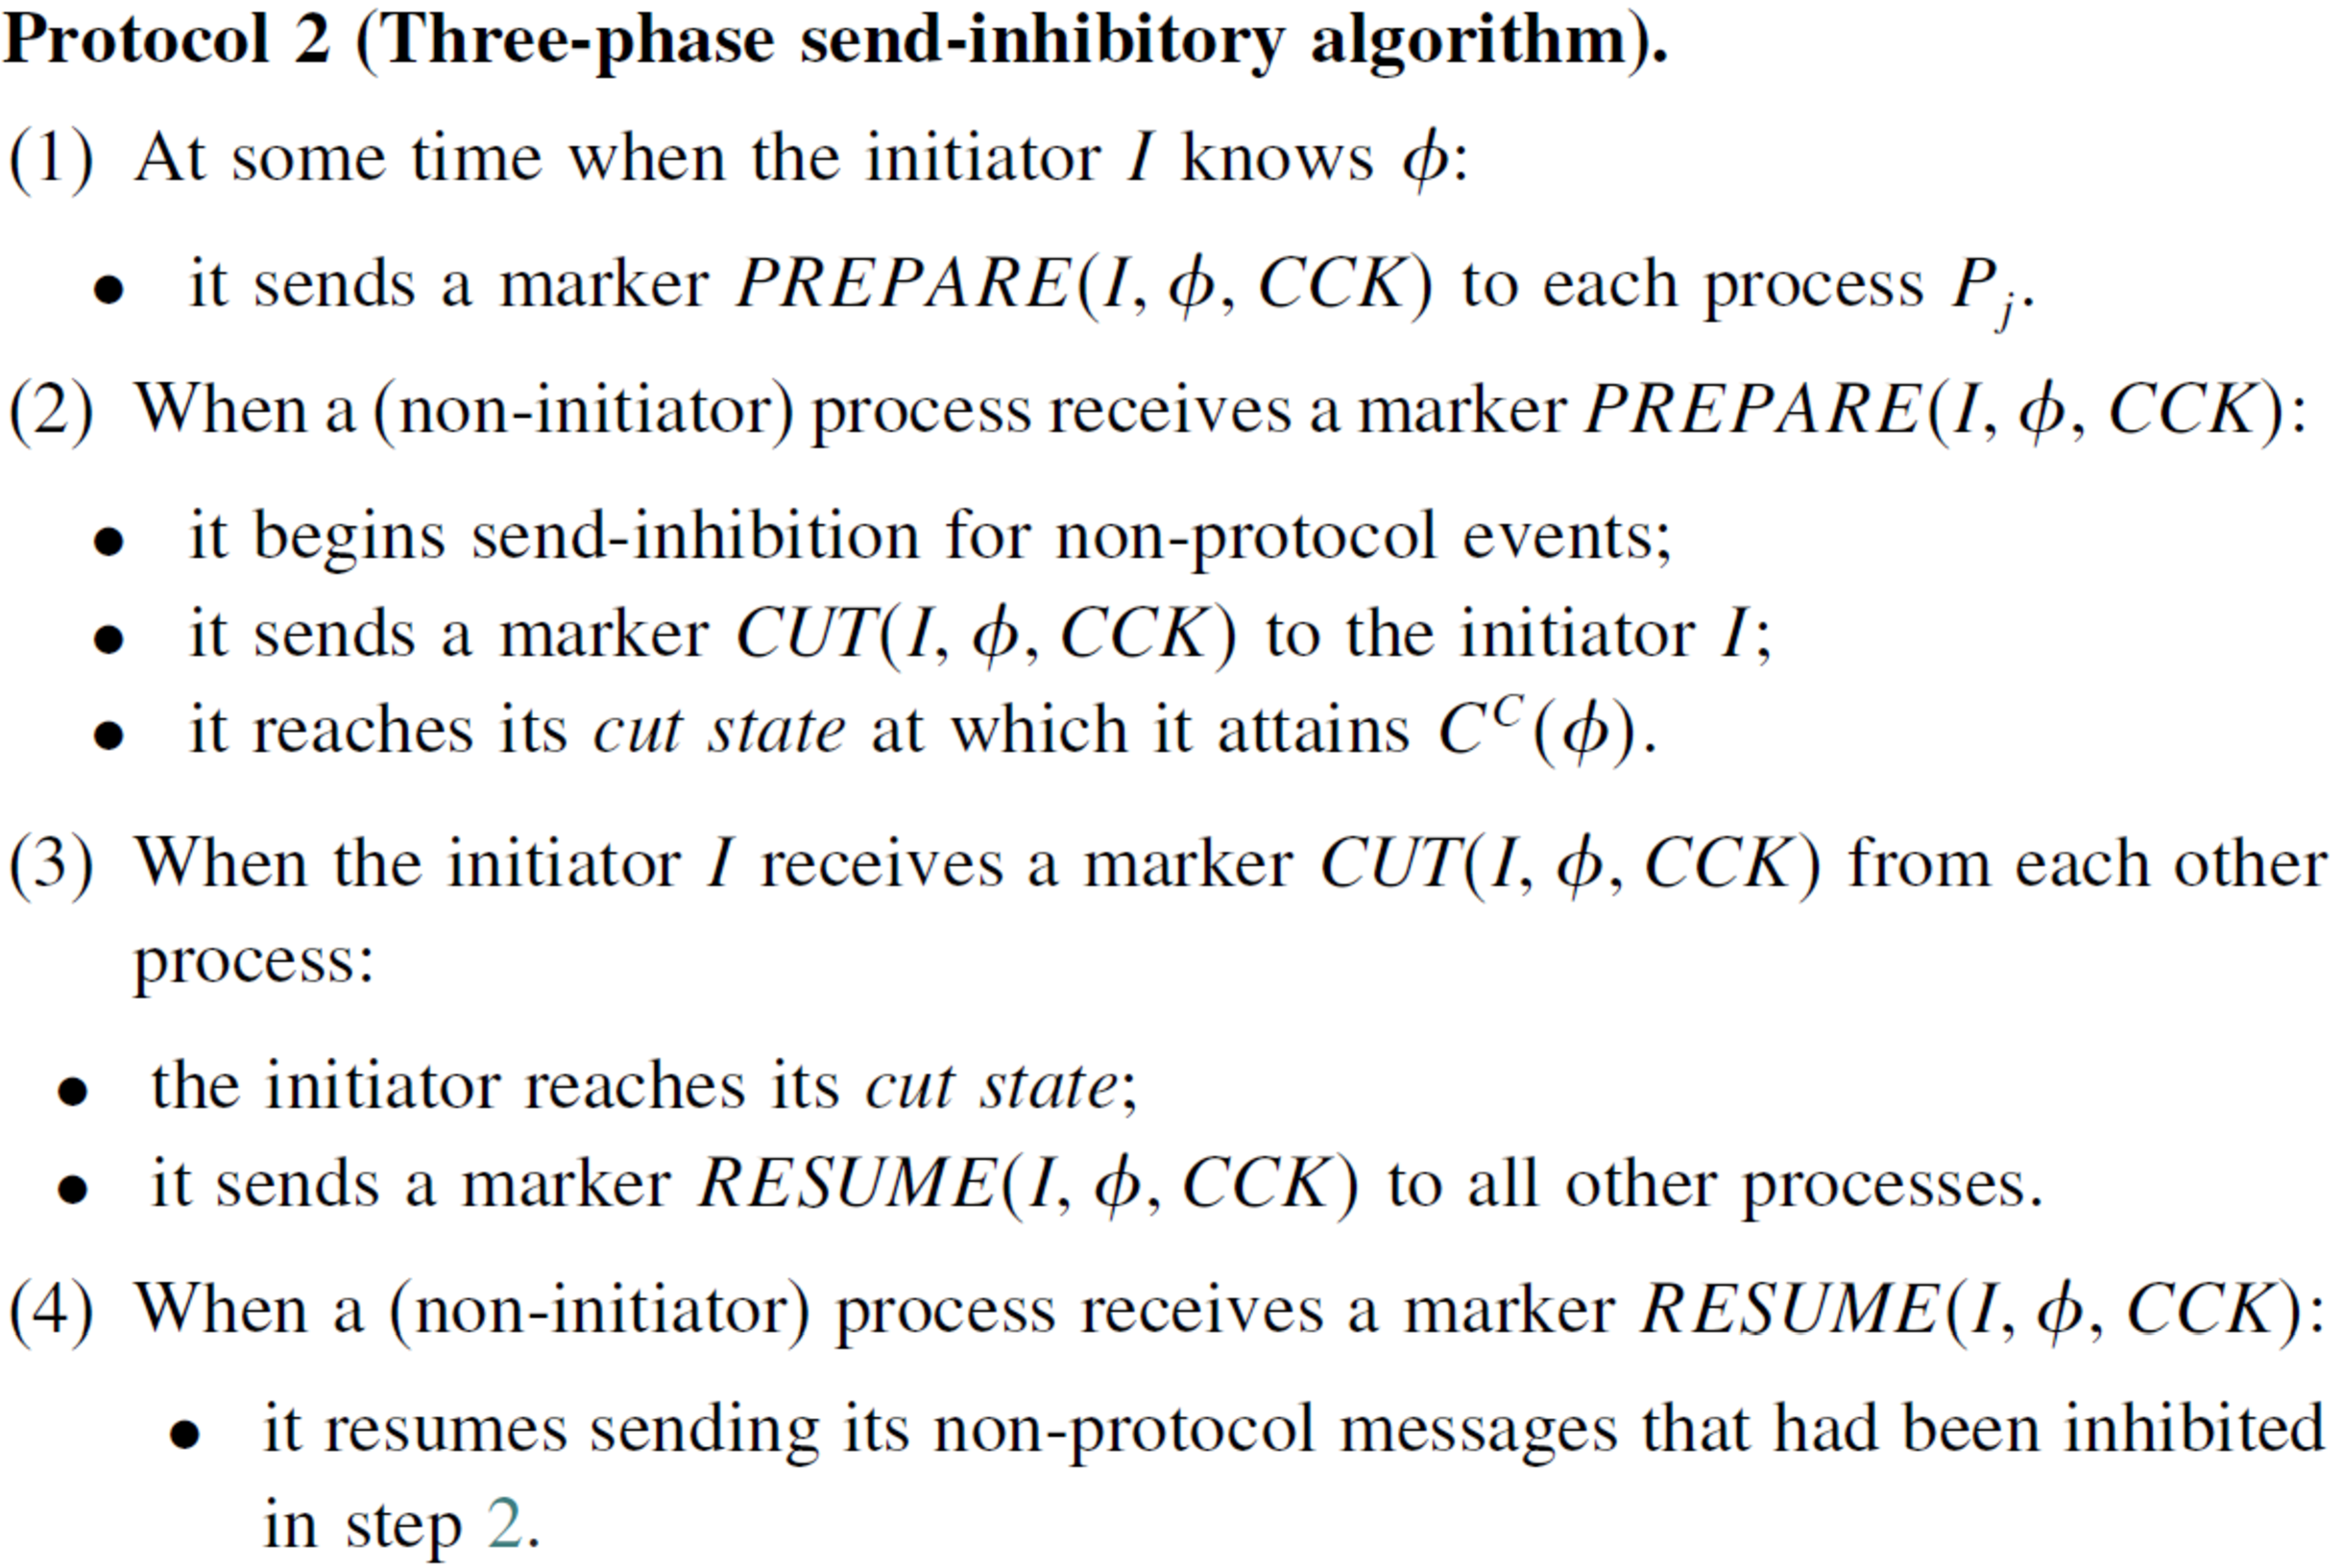
\includegraphics[width=1\textwidth]{three_phase_algo.pdf}
  \caption{ Drei-Phasen Algorithmus für die Gewährleistung von gleichzeitig gemeinsamen Wissen \cite{kshemkalyani2011distributed}}
\label{pic:lbsn}
\end{figure}
Durch den sogenannten Drei-Phasen Algorithmus (Abb. 4) wird gewährleistet, dass alle Prozesse einen Zustand erreichen, welcher einen sicheren und konsistenten Informationsaustausch dient. Er wird in 4 Schritte untergliedert:
\begin{enumerate}
\item Im ersten Schritt sendet ein Initiator eine Nachricht aus, um die anderen Prozesse auf einen Informationsaustausch vorzubereiten.
\item Nachdem der Prozess diese Nachricht erhalten hat, werden zunächst alle anderen Operationen gesperrt und ein konsistenter Zustand eingenommen, ehe der Initiator benachrichtigt wird, dass der Prozess bereit für einen Informationsaustausch ist.
\item Nachdem der Initiator von allen Prozessen benachrichtigt wurde, dass diese bereit für den Austausch sind, erreicht dieser selbst einen konsistenten Zustand und benachrichtigt die anderen.
\item Im letzten Schritt findet nun der eigentliche Nachrichtenaustausch statt. 
\end{enumerate}

Der Algorithmus ist sehr klar strukturiert und bietet die Möglichkeit von sicherer Übertragung von Informationen. So kann innerhalb von asynchronen Systemen mit Daten gearbeitet werden, welche auf gemeinsamen Wissen beruhen ohne das es Unsicherheiten im Bezug auf die Teilnehmer gibt. 